\documentclass{beamer}

\usepackage{array}
\usepackage[english]{babel}
\usepackage[utf8x]{inputenc}
\usepackage{amssymb}
\usepackage{amsmath}
\usepackage{geometry}
\usepackage{graphicx}
\usepackage{eucal}
\usepackage{cite}
\usepackage{wrapfig}
\usepackage{datetime}
\usepackage[font=small,labelfont=bf]{caption}

\graphicspath{ {./fig} }
\setbeamertemplate{bibliography item}{\insertbiblabel}

\title{Message integrity: secure hash functions and random numbers}
\author{Alexander Buchnev}

\newdateformat{monthYear}{\monthname[\THEMONTH] \THEYEAR}
\date{\monthYear\today}

\DeclareCaptionFormat{custom}
{%
    \textbf{\tiny #1#2}\textit{\tiny #3}
}
\captionsetup{format=custom}

\begin{document}

\frame{
	\titlepage
}

\newtheorem{prop}{Proposition}

%% Proof for the homework

\section*{Outline}

\begin{frame}{Outline}
	\tableofcontents
\end{frame}

\begin{frame}{Hash functions}
    \section{What is the hash function?}
    \begin{definition}[Hash function]
        Hash function (one way function, cryptographic hash function) is a 
        special type of function, which maps the arbitrary sized messages to 
        the fixed size values. 
    \end{definition}
    \begin{example}[Simple examples of hash function]
        \begin{itemize}
            \item reduction modulo $n$
            \item polynomial addition of string characters and then reduction 
            modulo $p$
            \item byte operations (most common)
            % \item hash functions built on top of encryption schemes
        \end{itemize}
    \end{example}
\end{frame}

\section{Cryptographic hash function}

\begin{frame}{Cryptographic hash function}
    What is the cryptographic hash function?
    \pause
    \begin{definition}[Cryptographic hash function]
        Cryptographic hash function is a hash function which satisfies the 
        following properties:
        \begin{itemize}
            \item \textbf{Preimage resistance.} Given the hash value $h$ is must be 
            infeasible to find such message $m$ that hashes to $h$.
            \pause
            \item \textbf{Second pre-image resistance.} Given an input $m1$ it 
            must be infeasible to find different $m2$ such that it has the 
            same hash value.
            \pause
            \item \textbf{Collision resistance.} Given nothing other than the 
            hash function itself, find 2 distinct inputs which will produce the 
            same hash value.
        \end{itemize}
    \end{definition}
\end{frame}

\begin{frame}{Other properties of hash functions\footnote{https://crypto.stackexchange.com/questions/55435/designing-a-hash-function-from-first-principles-rather-than-depending-on-heurist}}
    \begin{itemize}
        \item \textbf{Strict avalanche criterion.} If you change any bit (or 
        any sequence of bits), in the input, all bits in the output must have 
        50\% change to change too.
        \pause
        \item \textbf{Nonlinearity.} If the hash function is linear, one can 
        create the system of the linear equations and just solve it for the 
        arbitrary preimages. Take the already mentioned reduction modulo $n$
        for example. Let us modify it a bit, so the resulting equation looks 
        like this: $f(m) = a \cdot m + b \pmod n$. Then if we are given the 
        hash value $f(m)$, we can easily construct the message by solving the 
        equation: $m = a^{-1} \cdot (f(m) - b) \pmod n$. Although it is a toy 
        example, one can come up with more hard, but linear one, which is prone 
        to this method.
        \pause
        \item Another thing to consider is balance. You want your hash behave 
        like the so called random oracle. 
    \end{itemize}
\end{frame}

\section{Applications of (cryptographic) hash functions}

\begin{frame}{Applications of (cryptographic) hash functions}
    \begin{itemize}
        \item Message integrity check 
        \item Message authentification
        \item Hash Tables
        \item PoW (Proof of Work) blockchain networks
        \item etc.
    \end{itemize}
\end{frame}

\section{Cryptographic hash function cosntructions}

\begin{frame}{How can one construct the hash function?}
    Below I am going to talk about 2 constructions: Merkle-Damgård and the 
    Sponge construction. I chose these two because SHA1 and SHA2 were the NIST 
    standard functions that are based on the Merkle-Damgård construction, and 
    the SHA3 finalist (Keccak) is based on the Sponge construction, which is 
    completely different from the Merkle-Damgård and it is worth discussing 
    therefore.
\end{frame}

\subsection{Merkle-Damgård construction}

\begin{frame}{Merkle-Damgård construction}
    Some of the most used hash functions are based on Merkle-Damgård 
    construction:
    \begin{itemize}
        \item MD5
        \item SHA1, SHA2
    \end{itemize}
\end{frame}

\begin{frame}{Step-by-step description of the Merkle-Damgård construction}
    \begin{enumerate}
        \item Pad the initial message with the appropriate padding scheme 
        (in case of md5, it is 0x80 and a bunch of zeroes)
        \item Initialize the IV (input vector --- initial state)
        \item Process message in blocks
        \item Finalize
    \end{enumerate}
\end{frame}

\begin{frame}{Merkle-Damgård construction}
    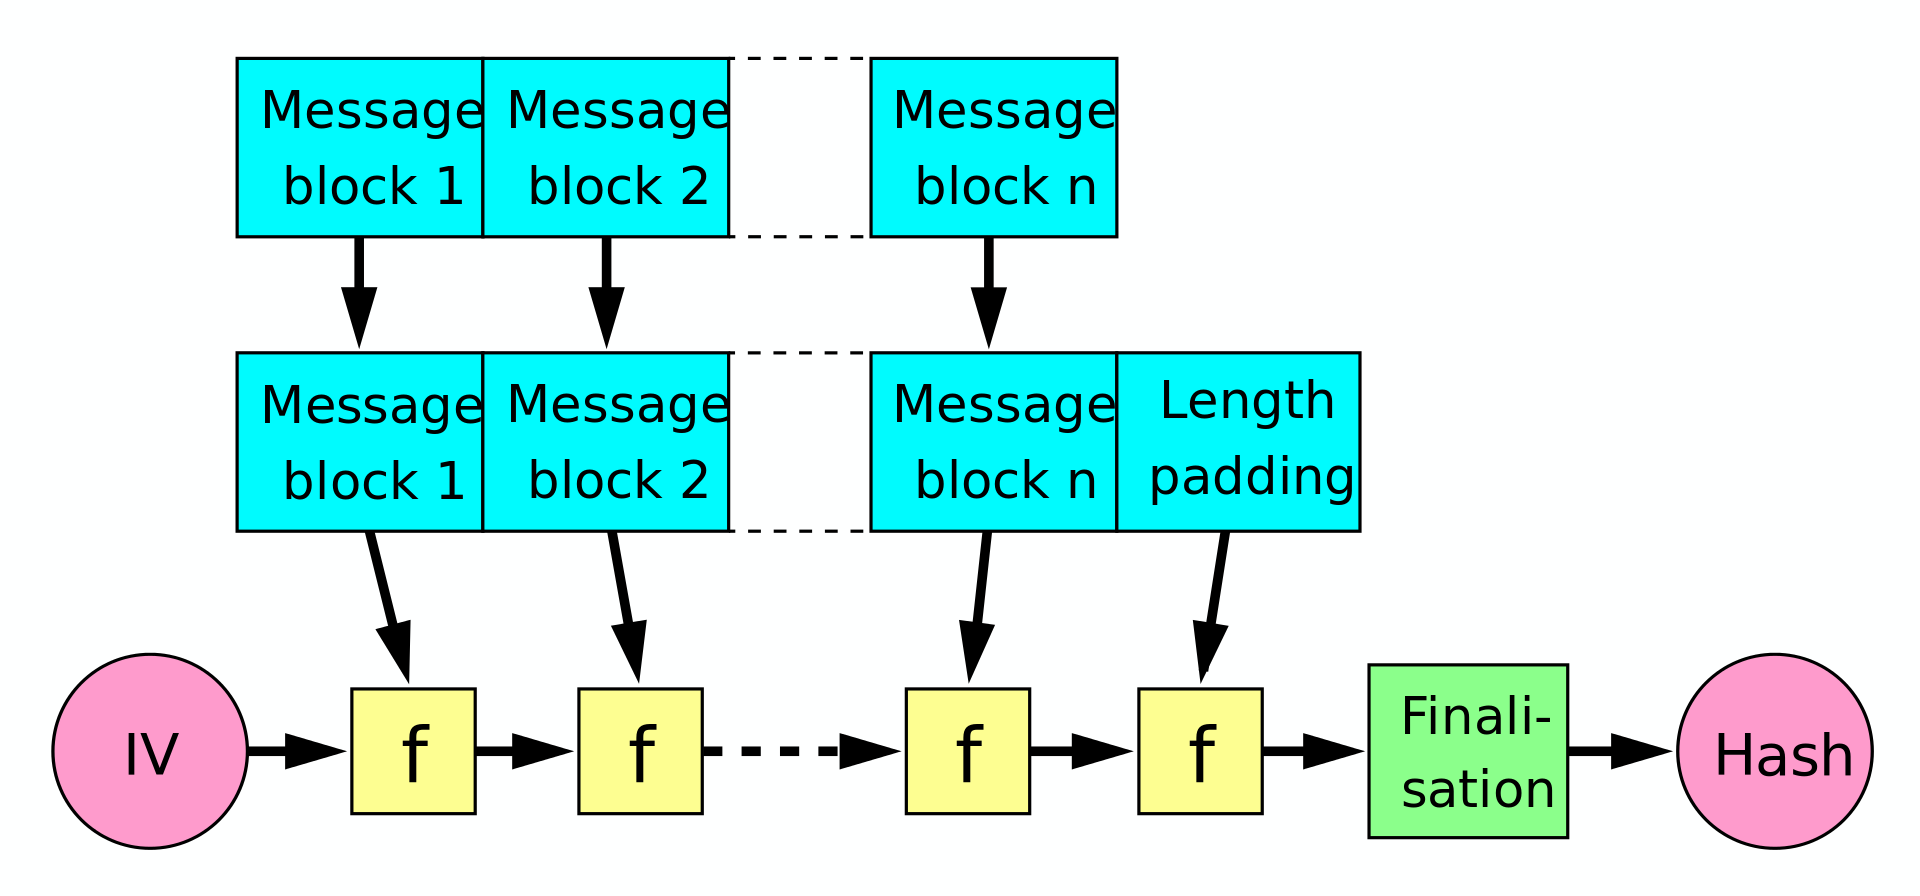
\includegraphics[width=\textwidth]{Merkle-Damgard_hash_big.svg.png}
    \captionof*{figure}{General Merkle-Damgård construction scheme. wikipedia.org}
\end{frame}

\subsection{Sponge construction}

\begin{frame}{Sponge construction}
    \par According to final version of FIPS 202 where the SHA3 is descibed, 
    SHA3 is the family of the functions on binary data. Each version of SHA-3 
    is based on the instance of the Keccak algorithm (family of the functions).
    Keccak is based on the Sponge construction. 
    \newline \newline
    \pause
    \par In Guido Bertoni and his team introduced the Sponge Construction. Simply 
    said, sponge function can take a message of the arbitrary length and 
    produce the hash digest of the desired length.
    \newline \newline
    \pause
    \par There are two phases of the Sponge function. First is called `absorbtion', 
    when the message is fed into the hash function, the second is when we 
    `squeeze' the result.
\end{frame}

\begin{frame}{Sponge Construction}
    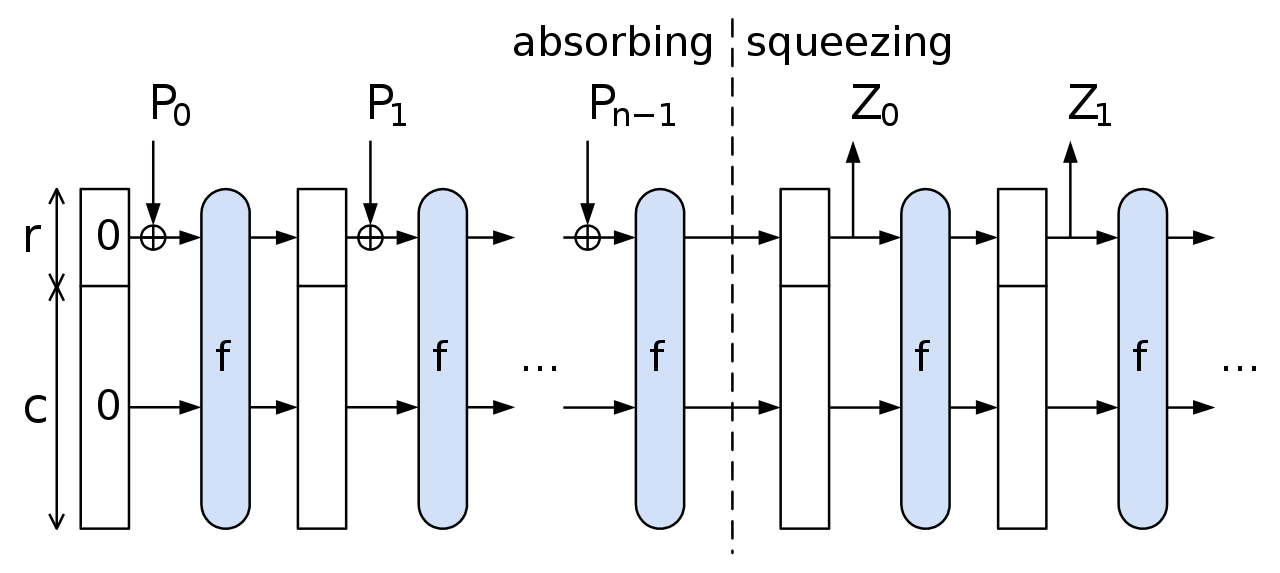
\includegraphics[width=0.8\textwidth]{SpongeConstruction.svg.png}
    \captionof{figure}{The Sponge Construction. wikipedia.org}
    Step by step process of absorbing phase:
    \begin{enumerate}
        \item SHA3 standard specifies the $r+c$ is $1600$
        \item Input message is padded to the multiple of $r$
        \item Input message is split into the $n$ block with each of length $r$
        \item For each input block we xor it with the current state of $r$, 
        then we apply \textbf{permutation function $f$} to the whole state
    \end{enumerate}
\end{frame}

\begin{frame}{Squeezing phase}
    In the squeezing phase, we do the same operations, except for the input 
    message part, i.e. we apply the \textbf{permutation function $f$} to the 
    state and get the first $r$ bits of the state as the message digest.
\end{frame}

\section{General attacks on hash primitives}

\begin{frame}{General attacks on hash primitives}
    \begin{itemize}
        \item Rainbow Tables (bruteforce)
        \item Birthday Attack
        \item Differential Cryptanalysis
        \item SAT Cryptanalysis
    \end{itemize}
\end{frame}

\section{Salts, passwords and databases}

\begin{frame}{Salt}
    \begin{definition}[Cryptographic salt]
        Salt is a (random) piece of data which is appended to the message to 
        create the different hash digest due to the strict avalanche criterion
        described above.
    \end{definition}
    \pause
    What are the benefits of `salting the passwords?'
    \pause
    The main benefit is that the salting helps protecting against the `rainbow
    table attacks', as well as protects passwords that occur multiple times in 
    a database, as a new salt is used for each password. 
\end{frame}

\section{Random number generators}

\begin{frame}{PRNG}
    \begin{definition}[PRNG - PseudoRandom Number Generator]
        \pause
        PRNG is an algorithm which generates the sequence of numbers with 
        properties approximate to the random numbers.
    \end{definition}
    \pause
    For now, there are no `perfect' PRNGs!!
\end{frame}

\begin{frame}{Ways to build the PRNG}
    
\end{frame}

\begin{frame}
    Its Jupyter Notebook time!
\end{frame}

% \begin{frame}[allowframebreaks]{References}
% 	\section*{References}
% 	\bibliography{refs}
% 	\bibliographystyle{ieeetr}
% \end{frame}

\end{document}
